%% Преамбула TeX-файла

% 1. Стиль и язык
\documentclass[utf8x, 12pt]{G7-32} % Стиль (по умолчанию будет 14pt)


% Остальные стандартные настройки убраны в preamble.inc.tex.
\sloppy

% Настройки стиля ГОСТ 7-32
% Для начала определяем, хотим мы или нет, чтобы рисунки и таблицы нумеровались в пределах раздела, или нам нужна сквозная нумерация.
\EqInChapter % формулы будут нумероваться в пределах раздела
\TableInChapter % таблицы будут нумероваться в пределах раздела
\PicInChapter % рисунки будут нумероваться в пределах раздела

% Добавляем гипертекстовое оглавление в PDF
\usepackage[
bookmarks=true, colorlinks=true, unicode=true,
urlcolor=black,linkcolor=black, anchorcolor=black,
citecolor=black, menucolor=black, filecolor=black,
]{hyperref}

% Изменение начертания шрифта --- после чего выглядит таймсоподобно.
% apt-get install scalable-cyrfonts-tex

\IfFileExists{cyrtimes.sty}
    {
        \usepackage{cyrtimespatched}
    }
    {
        % А если Times нету, то будет CM...
    }

\usepackage{graphicx}   % Пакет для включения рисунков
\DeclareGraphicsExtensions{.jpg,.pdf,.png}
% С такими оно полями оно работает по-умолчанию:
% \RequirePackage[left=20mm,right=10mm,top=20mm,bottom=20mm,headsep=0pt]{geometry}
% Если вас тошнит от поля в 10мм --- увеличивайте до 20-ти, ну и про переплёт не забывайте:
\geometry{right=20mm}
\geometry{left=30mm}


\usepackage{algorithm}
\usepackage{algpseudocode}

% Перевод плагина
\makeatletter
% Перевод данных об алгоритмах
\renewcommand{\listalgorithmname}{Список алгоритмов}
\floatname{algorithm}{Алгоритм}

%% Перевод команд псевдокода
%\algrenewcommand\algorithmicwhile{\textbf{До тех пока}}
%\algrenewcommand\algorithmicdo{\textbf{выполнять}}
%\algrenewcommand\algorithmicrepeat{\textbf{Повторять}}
%\algrenewcommand\algorithmicuntil{\textbf{Пока выполняется}}
%\algrenewcommand\algorithmicend{\textbf{Конец}}
%\algrenewcommand\algorithmicif{\textbf{Если}}
%\algrenewcommand\algorithmicelse{\textbf{иначе}}
%\algrenewcommand\algorithmicthen{\textbf{тогда}}
%\algrenewcommand\algorithmicfor{\textbf{Цикл}}
%\algrenewcommand\algorithmicforall{\textbf{Выполнить для всех}}
%\algrenewcommand\algorithmicfunction{\textbf{Функция}}
%\algrenewcommand\algorithmicprocedure{\textbf{Процедура}}
%\algrenewcommand\algorithmicloop{\textbf{Зациклить}}
%\algrenewcommand\algorithmicrequire{\textbf{Условия:}}
%\algrenewcommand\algorithmicensure{\textbf{Обеспечивающие условия:}}
%\algrenewcommand\algorithmicreturn{\textbf{Возвратить}}
%\algrenewtext{EndWhile}{\textbf{Конец цикла}}
%\algrenewtext{EndLoop}{\textbf{Конец зацикливания}}
%\algrenewtext{EndFor}{\textbf{Конец цикла}}
%\algrenewtext{EndFunction}{\textbf{Конец функции}}
%\algrenewtext{EndProcedure}{\textbf{Конец процедуры}}
%\algrenewtext{EndIf}{\textbf{Конец условия}}
%\algrenewtext{EndFor}{\textbf{Конец цикла}}
%\algrenewtext{BeginAlgorithm}{\textbf{Начало алгоритма}}
%\algrenewtext{EndAlgorithm}{\textbf{Конец алгоритма}}
%\algrenewtext{BeginBlock}{\textbf{Начало блока. }}
%\algrenewtext{EndBlock}{\textbf{Конец блока}}
%\algrenewtext{ElsIf}{\textbf{иначе если }}
\makeatother

%\usepackage{caption}
%\captionsetup[ruled]{labelsep=period}
%\makeatletter
%\@addtoreset{algorithm}{chapter}% algorithm counter resets every chapter
%\makeatother
%\renewcommand{\thealgorithm}{\thechapter.\arabic{algorithm}}% Algorithm # is %<chapter>.<algorithm>


% Произвольная нумерация списков.
\usepackage{enumerate}
\usepackage{color}

\usepackage{hyperref}
\usepackage{listings}
%\lstset{extendedchars=\true}
\lstset{ %
	language=[Auto]Lisp,
	inputencoding=cp1251,
	basicstyle=\small\sffamily, % размер и начертание шрифта для подсветки кода
	numbers=left,               % где поставить нумерацию строк (слева\справа)
	numberstyle=\tiny,           % размер шрифта для номеров строк
	stepnumber=1,                   % размер шага между двумя номерами строк
	numbersep=5pt,                % как далеко отстоят номера строк от подсвечиваемого кода
	backgroundcolor=\color{white}, % цвет фона подсветки - используем \usepackage{color}
	showspaces=false,            % показывать или нет пробелы специальными отступами
	showstringspaces=false,      % показывать или нет пробелы в строках
	showtabs=false,             % показывать или нет табуляцию в строках
	frame=single,              % рисовать рамку вокруг кода
	tabsize=2,                 % размер табуляции по умолчанию равен 2 пробелам
	captionpos=t,              % позиция заголовка вверху [t] или внизу [b] 
	breaklines=true,           % автоматически переносить строки (да\нет)
	breakatwhitespace=false, % переносить строки только если есть пробел
	escapeinside={-\%*}{*)}   % если нужно добавить комментарии в 
}
%\usepackage{minted}

\setcounter{tocdepth}{2} %Подробность оглавления
%4 это chapter, section, subsection, subsubsection и paragraph
%3 это chapter, section, subsection и subsubsection
%2 это chapter, section, и subsection
%1 это chapter и section
%0 это chapter.


\begin{document}
	\lstset{language=csh} 
	\frontmatter % выключает нумерацию ВСЕГО; здесь начинаются ненумерованные главы: реферат, введение, глоссарий, сокращения и прочее.
	\pagestyle{empty}
	{\Large Моделирование коррупции на основе игры в развернутой форме
\par}
{\large 
	Сычев Роман Сергеевич, математика  и компьютерные науки (кафедра математического анализа)\\
	Научный руководитель: Глазков Д.В., кандидат ф.-м. н., доцент
\par}
Данная работа рассматривает вопросы минимизации сожалений в игровых моделях коррупции на основе игр в развернутой форме. В работе приводится описание моделей и рассматриваются некоторые возможные программные реализации с применением методов объектно-ориентированного программирования.
\par
Работа включает три главы. 
\par
В первой главе приведено описание алгоритма CFR, который является адаптацией алгоритма минимизации сожалений для игр с неполной информацией. В главе приведены все основные определения и описана процедура минимизации контрафактических сожалений на основе алгоритма Блэквелла. Алгоритм рассматривает конечные игры в развернутой форме с неполной информацией. Реализуется итеративная процедуру, на каждом шаге которой обновляется профиль стратегий игроков. После любого числа итераций можно оценить качество полученных стратегических профилей, вычислив сумму сожалений игроков.
\par
Во второй главе приведено описание двух игровых моделей коррупции. В качестве первого примера выбрана модель раскрытия совместного преступления, и модель коррупции в иерархической структуре в качестве второго примера. Модель раскрытия совместного реализует механизм подкупа чиновника клиентом с возможной проверкой обоих инспектором. Модель коррупции в иерархической структуре использует похожие механизмы распределения информации между игроками, но уже для случая иерархии сотрудников. Основным отличием является возможность разоблачения руководителя, для смягчения собственного наказания. Обе модели предусматривают асимметричные выплаты игрокам.
\par
В третьей главе приведено описание реализации алгоритма CFR для двух игровых моделей коррупции. Для каждой модели приведено описание в соответствии с определениями из первой главы. Для иллюстрации работы алгоритма приведены некоторые результаты работы соответствующих программ, часть кода которых представлена в приложениях.
\par
В заключении сделаны выводы о проделанной работе и подведен итог исследованию. В ходе работы была получена программная реализация минимизации сожалений для двух задач моделирования коррупции.
	\begin{center}
	{\large \textbf{Реферат}}
\end{center}
\par
Дипломная работа <<Моделирование коррупции на основе игры в развернутой форме>> 54 стр., 5 таблиц, 13 илл., 8 источников, 3 прил.
\par
Ключевые слова: теория игр, искусственный интеллект, моделирование коррупции, неполная информация, игры в развернутой форме.
\par
Объектом исследования являются игровые модели коррупции на основе игр в развернутой форме.
\par
Целью работы является программная реализация минимизации сожалений для игровых моделей коррупции.
\par
В данной работе была рассмотрена реализация минимизации сожалений для некоторых задач моделирования коррупции.
Полученные в результате работы программные классы могут использоваться для практического расчета. К преимуществам полученной иерархической модели можно отнести масштабируемость с точки зрения проверяемых лиц и свободный выбор альтернатив игроками. Полученные алгоритмы и методики могут быть использованы как для изучения старых, так и для построения новых моделей и абстракций.
	\pagestyle{plain}
	\begin{center}
	\large{МИНИСТЕРСТВО НАУКИ И ВЫСШЕГО ОБРАЗОВАНИЯ РОССИЙСКОЙ ФЕДЕРАЦИИ}\\
	\footnotesize{ФЕДЕРАЛЬНОЕ ГОСУДАРСТВЕННОЕ БЮДЖЕТНОЕ ОБРАЗОВАТЕЛЬНОЕ УЧРЕЖДЕНИЕ}\\ 
	\footnotesize{ВЫСШЕГО ОБРАЗОВАНИЯ}\\
	\small{\textbf{«Ярославский государственный университет им. П.Г. Демидова»}}\\
	\hfill \break
	\hfill\break
	\hfill \break
	\hfill \break
	\hfill \break
	\hfill \break
	\hfill \break
	\hfill \break
	\hfill \break
	\hfill \break
	
	\normalsize{Выпускная квалификационная работа}\\
	\large{Моделирование коррупции на основе игры в развернутой форме}\\	
	02.04.01. Математика и компьютерные науки\\
	
	\hfill \break
	\hfill \break
	\hfill \break
	\hfill \break
	\hfill \break
\end{center}

\normalsize{ 
	\begin{flushleft}
		\hspace*{80mm}Исполнитель: Сычев Р.С. \\
		\hspace*{80mm}гр. МКН-21 МО \\
		\hspace*{80mm}Руководитель: к.ф.-м.н. Глазков Д.В.
	\end{flushleft}
}
\hfill \break
\hfill \break
\hfill \break
\hfill \break
\hfill \break
\hfill \break
\begin{center} Ярославль 2022 \end{center}
\thispagestyle{empty} % выключаем отображение номера для этой страницы

	
	\thispagestyle{empty}
	\setcounter{page}{0}
	\tableofcontents
	\clearpage
	
	
	\Introduction

\par
В последнее время математическая теория игр с неполной информацией находит все большее применение в таких отраслях как теория операций, экономика, кибербезопасность и физическая безопасность. Не в последнюю очередь это происходит благодаря постоянному совершенствованию алгоритмов и увеличению производительности вычислительной техники. Частным случаем таких игр являются игры в развернутой форме. При такой постановке задачи можно близким к естественному способом отразить в игровой форме структуру последовательного принятия решений набором участников в конфликтной ситуации.
\par
Существенным шагом в развитии данного направления является использование алгоритма подсчета сожалений (regret matching). Алгоритм предполагает итеративное вычисление последовательности стратегий в среднем сходящейся к оптимальному стратегическому профилю. Открытие этого метода привело к появлению ряда алгоритмов для поиска приближенного решения в играх с неполной информацией.
\par
Данная работа посвящена рассмотрению одного из популярных в настоящее время итеративных алгоритмов -  контерфактической минимизации сожалений (Conterfactual Regret Minimization) и его модификации приедусматривающей использование метода монте карло (MCCFR). Данные алгоритмы появились не так давно, но на их основе уже получен ряд недостижимых до этого по сложности результатов. 
\par
Целью данной работы является описание и отработка на практике приведенных выше алгоритмов.
\par
В соответствии с темой работы поставлены следующие задачи:
\begin{itemize}
	\item подготовить теоритическое описание алгоритмов;
	\item выделить некоторые игры в развернутой форме для последующего решения;
	\item реализовать алгоритм и произвести расчет стратегического профиля для приведенных игр.
\end{itemize}
\par
Данная работа может быть интересна людям желающим ознакомится с некоторыми современными техниками решения игр с неполной информацией.

	
	\mainmatter
	
	\chapter{Термины, определения и обозначения}
\label{cha:ch_1}
\newcounter{MYc} 
\def\MYhyp{\addtocounter{MYc}{1}{\bf Определение \arabic{MYc}: }}
\par
В настоящей дипломной работе применяются следующие термины и обозначения с соответствующими определениями.
\par
\textbf{Дополнение} "--- приписывание дополнительных бит к строке бит.
\par
\textbf{Инициализационный вектор} "--- вектор, определенный как начальная точка работы функции хэширования.
\par
\textbf{Ключ подписи} "--- элемент секретных данных, специфичный для субъекта и используемый только данным субъектом в процессе формирования цифровой подписи.
\par
\textbf{Ключ проверки подписи} "--- элемент данных, математически связанный с ключом подписи и используемый проверяющей стороной в процессе проверки цифровой подписи.
\par
\textbf{Параметр схемы ЭЦП} "--- элемент данных, общий для всех субъектов схемы цифровой подписи, известный или доступный всем этим субъектам.
\par
\textbf{Подписанное сообщение} "--- набор элементов данных, состоящий из сообщения и дополнения, являющегося частью сообщения.
\par
\textbf{Последовательность псевдослучайных чисел} "--- последовательность чисел, полученная в результате выполнения некоторого арифметического (вычислительного) процесса, используемая в конкретном случае вместо последовательности случайных чисел.
\par
\textbf{Последовательность случайных чисел} "--- последовательность чисел, каждое из которых не может быть предсказано (вычислено) только на основе знания предшествующих ему чисел данной последовательности.
\par
\textbf{Процесс проверки подписи} "--- процесс, в качестве исходных данных которого используются подписанное сообщение, ключ проверки подписи и параметры схемы ЭЦП, результатом которого является заключение о правильности или ошибочности цифровой подписи.
\par
\textbf{Процесс формирования подписи} "--- процесс, в качестве исходных данных которого используются сообщение, ключ подписи и параметры схемы ЭЦП, а в результате формируется цифровая подпись.
\par
\textbf{Свидетельство} "--- элемент данных, представляющий соответствующее доказательство достоверности (недостоверности) подписи проверяющей стороне.
\par
\textbf{Случайное число} "--- число, выбранное из определенного набора чисел таким образом, что каждое число из данного набора может быть выбрано с одинаковой вероятностью.
\par
\textbf{Сообщение} "--- строка бит произвольной конечной длины.
\par
\textbf{Функция сжатия} "--- итеративно используемая функция, преобразующая строку бит длиной $L_1$ и полученную на предыдущем шаге строку бит длиной $L_2$ в строку бит длиной $L_2$.
\par
\textbf{Хэш-код} "--- строка бит, являющаяся выходным результатом хэш-функции.
\par
\textbf{Хэш-функция} "--- функция, отображающая строки бит в строки бит фиксированной длины и удовлетворяющая следующим свойствам:
\begin{enumerate}
	\item по данному значению функции сложно вычислить исходные данные, отображаемые в это значение;
	\item для заданных исходных данных сложно вычислить другие исходные данные, отображаемые в то же значение функции;
	\item сложно вычислить какую-либо пару исходных данных, отображаемых в одно и то же значение.
\end{enumerate}
\par
\textbf{Электронная цифровая подпись (ЭЦП)} "--- строка бит, полученная в результате процесса формирования подписи.
\par
$V^*$ "--- множество всех двоичных векторов-строк конечной размерности (далее - векторы), включая пустую строку.
\par
$|A|$"--- размерность (число компонент) вектора $A\in V^*$ (если $A$ - пустая строка, то $|A|=0$).
\par
$V_n$ "--- множество всех $n$-мерных двоичных векторов, где $n$ - целое неотрицательное число; нумерация подвекторов и компонент вектора осуществляется справа налево, начиная с нуля.
\par
$\oplus$ "--- операция покомпонентного сложения по модулю 2 двух двоичных векторов одинаковой размерности.
\par
$A\|B$ "--- конкатенация векторов $A,B\in V^*$, т.е. вектор из $V_{|A|+|B|}$, в котором левый подвектор из $V_{|A|}$ совпадает с вектором $А$, а правый подвектор из $V_{|B|}$ совпадает с вектором $В$.
\par
$A^n$ "--- конкатенация $n$  экземпляров вектора $A$.
\par
$\mathbb{Z}_{2^n}$ "--- кольцо вычетов по модулю $2^n$.
\par
$\boxplus$ "--- операция сложения в кольце $\mathbb{Z}_{2^n}$.
\par
$Vec_n:\mathbb{Z}_{2^n} \to V_n$ "--- биективное отображение, сопоставляющее элементу кольца $\mathbb{Z}_{2^n}$ его двоичное представление, т.е. для любого элемента $z \in \mathbb{Z}_{2^n}$ представленного вычетом $z_0+2z_1 + \dots 2^{n-1}z_{n-1}$, где $z_j \in \{0,1\},\,j=0,\dots,n-1$, выполнено равенство $Vec_n(z)=z_{n-1}\|\dots\|z_1\|z_0$.
\par
$Int_n\colon V_n \to \mathbb{Z}_{2^n}$ "--- отображение, обратное отображению $Vec_n$, т.е. \\ $Int_n = Vec_n^{-1}$.
\par
$MSB_n\colon V^* \to V_n$ "--- отображение, ставящее в соответствие вектору \\ $z_{k-1}\|\dots\|z_1\|z_0,\:k\geqslant n$, вектор $z_{k-1}\|\dots\|z_{k-n+1}\|z_{k-n}$.
\par
$a:=b$ "--- операция присваивания переменной $a$ значения $b$.
\par
$\Phi\circ\Psi$ "--- произведение отображений, при котором отображение $\Psi$ действует первым.
\par
$M$ "--- двоичный вектор, подлежащий хэшированию, $M \in V^*,\; |M|<2^{512}$.
\par
$H \colon V^* \to V_n$ "--- функция хэширования, отображающая вектор (сообщение) $M$ в вектор (хэш-код) $H(M)$.
\par
$IV$ "--- инициализационный вектор функции хэширования, $IV \in V_{512}$.
\par
$Z$ "--- множество всех целых цисел.
\par
$p$ "--- простое число, $p>3$.
\par
$F_p$ "--- конечное простое поле, представленное как множество  из $p$ наименьших неотрицательных вычетов $\{0,\;1,\;\dots,\;p-1\}$.
\par
$b\;(mod\; p)$ "--- минимальное неотрицательное число, сравнимое с $b$ по модулю $p$.
%\par
%$a, b$ "--- коэффициенты эллиптической кривой;
%\par
%$m$ "--- порядок группы точек эллиптической кривой;
%\par
%$q$ "--- порядок подгруппы группы точек эллиптической кривой;
%\par
%$O$ "--- нулевая точка эллиптической кривой;
%\par
%$P$ "--- точка эллиптической кривой порядка $q$;
%\par 
%$d$ "--- целое число "--- ключ подписи;
%\par
%$Q$ "--- точка эллиптической кривой "--- ключ проверки подписи;
%\par
%$\zeta$ "--- цифровая подпись над сообщением $M$;


	\chapter{Первая глава. Описание алгоритмов}
\label{cha:ch_1}
\section{Игры в развернутой форме и равновесие}
\par
Игра в развернутой форме представляют компактную общую модель взаимодействий между агентами и явно отражает последовательный характер этих взаимодействий. Последовательность принятия решений игроками в такой постановке представлена деревом решения. При этом, листья дерева отождествлены с терминальными состояниями, в которых игра завершается и игроки получают выплаты. Любой нетерминальный узел дерева представляет точку принятия решения. Неполнота информации выражается в том, что различные узлы игрового дерева считаются неразличимыми для игрока. Совокупность всех попарно неразличимых состояний игры называется информационными состояниями. Приведем формальное определение.
\par
\begin{defin}\label{def1}
Конечная игра в развернутой форме с неполной информацией содержит следующие компоненты:
\end{defin}
\begin{itemize}
	\item конечное множество игроков $N$;
	\item конечное множество историй действий игроков $H$, такое, что $\emptyset \in H$ и любой префикс элемента из $H$ также принадлежит $H$. $Z \subseteq H$ представляет множество терминальных историй (множество историй игры на являющихся префиксом). $A(h)=\{a \colon (h,\;a)\in H \}$ "--- доступные после нетерминальной истории $h\in H$ действия;
	\item функция $P\colon H\setminus Z \to N \cup \{c\}$, которая сопоставляет каждой нетерминальной истории $h\in H\setminus Z$ игрока, которому предстоит принять решение, либо игрока $c$ представляющего случайное событие;
	\item функция $f_c$, которая сопоставляет всем $h \in H$, для которых $P(h)=c$, вероятностное распределение $f_c(\cdot |h)$ на $A(h)$. $f_c(a|h)$ представляет вероятность выбора $a$ после истории $h$;
	\item для каждого игрока $i \in N$ $\mathcal{I}_i $ обозначает разбиение $ \{h \in H \colon P(h) = i\}$, для которого $A(h)=A(h')$ всякий раз когда $h$ и $h'$ принадлежат одному элементу разбиения. Для $I_i \in \mathcal{I}_i$ определим $A(I_i)=A(h)$ и $P(I_i)=i$ для всех $h \in I_i$. $\mathcal{I}_i$ называют информационным набором игрока $i$, а $I_i \in \mathcal{I}_i$ информационным состоянием игрока $i$;
	\item для каждого игрока $i \in N$ определена функция выигрыша $u_i \colon Z \to \mathbb{R}$. Если для игры в развернутой форме выполняется $\forall z \in Z \sum_{i \in N}U_i(z) = 0 $, то такую игру называют игрой с нулевой суммой. Определим $\Delta_{u,i} = max_{z\in Z}\;u_i(z) - min_{z\in Z}\;u_i(z)$ для диапазона выплат игрока. 
\end{itemize}
\par
 Отметим, что информационные наборы могут использоваться не только для реализации правил конкретной игры, но и могут быть использованы для того, чтобы заставить игрока забыть о предыдущих действиях. Игры в которых игроки не забывают о действиях называют играми с полной памятью. В дальнейшем мы будем рассматривать конечные игры в развернутой форме с полной памятью.

Стратегия игрока $i$ "--- это функция $\sigma_i$, которая ставит в соответствие каждому информационному состоянию $I_i \in \mathcal{I}_i$ вероятностное распределение на $A(I_i)$. Обозначим за $\Sigma_i$ множество всех стратегий игрока $i$. Стратегический профиль $\sigma$ содержит стратегии для каждого игрока $i \in N$. При этом за $\sigma_{-i}$ обозначим $\sigma$ без $\sigma_i$. 

Обозначим за $\pi^\sigma(h)$ вероятность того, что игроки достигнут $h$ руководствуясь $\sigma$. Мы можем представить $\pi^\sigma$ как $\pi^\sigma = \prod_{i\in N\cup\{c\}}\pi_i^\sigma(h)$, выделяя вклад каждого игрока. В таком случае, $\pi_i^\sigma(h)$ обозначает вероятность принятия совокупности решений игрока $i$, ведущих от $\emptyset$ к $h$. Иными словами
\begin{equation*} 
\pi_i^\sigma(h)=
\begin{cases}
	\prod_{h \sqsubset h' \wedge P(h')=i \wedge h \sqsubset (h',a)} \sigma(h')(a) & \{h' | h \sqsubset h' \wedge P(h')=i \} \neq \emptyset\\
	1 &\text{иначе.}
\end{cases}
\end{equation*}
Запись $h \sqsubset h'$ означает, что $h'$ является префиксом $h$. 
Обозначим за $\pi_{-i}^\sigma(h) $ вероятность достижения истории $h$ всеми игроками (включая $c$) за исключением $i$.
Для $I \subseteq H $ определим $\pi^\sigma(I) = \sum_{h\in I}\pi^\sigma(h)$. Аналогично, введем $\pi_i^\sigma(I)$ и $\pi_{-i}^\sigma(I)$. 
\par
Ожидаемое значение выплаты для игрока $i$ обозначим как $u_i(\sigma)=\sum_{h\in Z}u_i(h)\pi^\sigma(h)$. 

Традиционным способом решения игр в развернутой форме является поиск равновесного профиля стратегий $\sigma$, который удовлетворяет следующему условию 
\begin{equation}
\begin{split}
	\forall i \in N,\;\;u_i(\sigma)\geq \underset{\sigma'_i\in \Sigma_i}{\max\;} u_i(\sigma'_i,\;\sigma_{-i}).
\end{split}
\end{equation} 
Такой стратегический профиль называют равновесием по Нэшу. В случае, если стратегический профиль $\sigma$ удовлетворяет условию 
\begin{equation}
	\begin{split}
		\forall i \in N,\; \epsilon > 0, \;\;u_i(\sigma) + \epsilon \geq \underset{\sigma'_i\in \Sigma_i}{\max\;} u_i(\sigma'_i,\;\sigma_{-i}).
	\end{split}
\end{equation}
его называют $\epsilon$ – равновесием по Нэшу.
\par
Для рассматриваемых далее алгоритмов наиболее интересен вариант игры с нулевой семмой для двух игроков. Именно для него имеется строгое математическое обоснование сходимости к равновесию Нэша.

\section{Контрафактические сожаления и их минимизация}

Минимизация сожалений является популярным концептом, для построения итеративных алгоритмов приближенного решения игр в развернутой форме \cite{RegretMatching}. Приведем связанные с ней определения. Рассмотрим дискретный отрезок времени $T$ включающий $T$ раундов от $1$ до $T$. Обозначим за $\sigma_i^t$ стратегию игрока $i$ в раунде $t$. 
\begin{defin}
	Средним общим сожалением игрока $i$ на момент времени $T$ называют величину 
\end{defin}
\begin{equation}
	R_i^T=\frac{1}{T} \underset{\sigma_i^*\in \Sigma_i}{\max\;}\sum_{t=1}^{T}u_i(\sigma_i^* ,\;\sigma_{-i}^t)-u_i(\sigma^t)
\end{equation} 

В дополнении к этому, определим $\bar{\sigma}_i^T$ как среднюю стратегию относительно всех раундов от 1 до T. Таким образом для каждого $I \in \mathcal{I}_i$ и $a\in A(I)$ определим 
\begin{equation}
	\bar{\sigma}_i^T(I)=\frac{\sum^T_{t=1}\pi_i^{\sigma^t}(I)\sigma^t(I)(a)}{\sum_{t=1}^{T}\pi_i^{\sigma^t}(I)}.
\end{equation}
\begin{theo} Если для игры с двумя игроками и с нулевой суммой на момент времени $T$ средние общие сожаления игроков меньше $\epsilon$, то $\sigma$ является $2\epsilon$ равновесием \cite{NIPS07cfr}. 
\end{theo}

Говорят, что алгоритм выбора $\sigma^t$ реализует минимизацию сожалений, если средние общие сожаления игроков стремятся к нулю при $t$ стремящимся к бесконечности. И как результат, алгоритм минимизации сожалений может быть использован для нахождения приближенного равновесия по Нэшу, в случае игр двух игроков с нулевой суммой. Вообще говоря, в случае ненулевой суммы или большего числа игроков алгоритм минимизации сожалений не приводит к равновесию Нэша. Однако, он приводит к другому классу равновесий. Доказано, что полученное решение сходится к грубому коррелированному равновесию и, более того,  устраняет итеративно доминируемые действия в профилях стратегий\cite{RGibson}.

Понятие контрафактического сожаления служит для декомпозиции среднего общего сожаления в набор дополнительных сожалений, которые могут быть минимизированы независимо для каждого информационного состояния. 

Обозначим через $u_i(\sigma,\;h)$ цену игры с точки зрения истории $h$, при условии, что $h$ была достигнута, и игроки спользуют в дальнейшем $\sigma$. 

\begin{defin}
	Контрафактической ценой $u_i(\sigma,\;I)$ назовем ожидаемую цену, при условии, что информационное состояние $I$ было достигнуто, когда все игроки кроме $i$ играли в соответствии с $\sigma$. Формально 
\end{defin} 
\begin{equation}
	u_i(\sigma,\;I)=\sum_{h\in I,h'\in Z}\pi_{-i}^\sigma(h)\pi^\sigma(h,\;h')u_i(h'),
\end{equation}
где $\pi^\sigma(h,\;h')$ "--- вероятность перехода из $h$ в $h'$.

Обозначим за $\sigma^t |_{I \to a}$ стратегический профиль идентичный $\sigma$ за исключением того, что $i$ всегда выбирает $a$ в $I$. 

Средним немедленным контрафактическим сожалением назовем 

\begin{equation}\label{Sych_eq1}
	R_{i,imm}^T(I) = \frac{1}{T}\underset{a\in A(I)}{\max\;}\sum_{t=1}^{T}u_i(\sigma^t |_{I \to a},\;I)-u_i(\sigma^t,\;I).
\end{equation}

Интуитивно это выражение можно понимать как аналог среднего общего сожаления в терминах контрафактической цены. Однако, вместо рассмотрения всевозможных максимизирующих стратегий рассматриваются локальные модификации стратегии. Положим $R_{i,imm}^{T,+}(I) = \max (R_{i,imm}^{T}(I),\;0)$. Связь немедленных контрафактических сожалений и общих средних сожалений раскрывает следующая теорема. 

\begin{theo} 
	$R_i^T \leq \sum_{I\in \mathcal{I}_i}R_{i,imm}^{T,+}(I)$\cite{NIPS07cfr}.
\end{theo}

Минимизация средних немедленных контрафактических сожалений приводит к минимизации средних общих сожалений. В свою очередь, минимизация среднего немедленного контрафактического сожаления может происходить за счет минимизации выражений под функцией максимума. Таким образом, мы приходим к понятию среднего контрафактического сожаления 
\begin{equation}
	R_i^T(I,\; a) = \frac{1}{T}\sum_{t=1}^{T}u_i(\sigma^t |_{I \to a},\;I)-u_i(\sigma^t,\;I).
\end{equation}
Контрафактическое сожаление рассматривает действие в информационном состоянии. В свою очередь, для минимизации средних контрафактических сожалений можно применить алгоритм приближения Блэквела\cite{RegretMatching}, который приведет к следующей последовательности стратегий 

\begin{equation}\label{CfrTStrategy}
	\sigma_i^{T+1}(I)(a)= 
	\begin{cases}
		\frac{R_i^{T,+}(I,\;a)}{\sum_{a\in A(I)}R_i^{T,+}(I,\;a)} &\text{если $\sum_{a\in A(I)}R_i^{T,+}(I,\;a) > 0$,}\\
		\frac{1}{|A(I)|} &\text{иначе.}
	\end{cases}
\end{equation}

Другими словами, действие выбирается в пропорции соотношения позитивных контрафактических сожалений о не выборе этого действия. Обоснование сходимости полученного решения и оценку ее скорости предоставляет следующая теорема. 

\begin{theo}\label{CfrTStrategyExp}
	 Если игроки придерживаются стратегий, заданных выражением (\ref{CfrTStrategy}), то $R_{i,imm}^T(I) \leq \Delta_{u,i}\sqrt{|A_i|}/\sqrt{T}$ и следовательно $R_i^T \leq \Delta_{u,i}|\mathcal{I}_i|\sqrt{|A_i|}/\sqrt{T}$, где $|A_i|=\max_{h\colon P(h)=i}|A(h)|$\cite{NIPS07cfr}.
\end{theo}

\par
Таким образом, по мере увеличения числа проведенных итераций уменьшаются средние общие сожаления.
	\chapter{Вторая глава. Программная реализация алгоритма}
\label{cha:ch_2}
\section{Общая схема вычислений}

\par
В рассмотренных далее примерах рассматривалась вероятностная реализация алгоритма MCCFR. При использовании данного метода значения случайных событий генерируются перед началом каждой обучающей итерации. Данный подход позволяет сократить обьем памяти и ускорить вычисления в некоторых случаях\cite{MCCFR}.
При реализации примеров были выделены следующие компоненты:
\begin{itemize}
	\item настройки игры (произвольная параметризация составных частей игры);
	\item описание правил игры (зависит от настроек);
	\item модуль с реализацией алгоритма относительно определенных правил и настроек.
\end{itemize}
\par
Настройки игры, например, по возможности могут включать число игроков, состав костяшек домино и т.п.
\par
Правила игры включают структуру игрового дерева, механизм распределения случайных событий и функцию выплат. Игровое дерево строится с применением узлов -- обьектов с информацией о историии игры, о игроке и о возможных действиях.
\par
Сам расчет итераций CFR происходит в выделенном модуле, на основе, определенных для каждого конкретного случая, правил игры. Работа алгоритма начинается с создания игрового дерева. Далее происходит расчет заданного числа итераций. После любой итерации можно получить средние стратегии игроков, которые представляют из себя приближенное коррелирующее равновесие.
\section{Первый пример. Покер Куна}

Покер Куна – это максимально упрощенная версия карточной игры покер\cite{KuhnPoker}.

Данная игра достаточно проста, чтобы быть решенной аналитически. Правила следующие:
\begin{itemize}
	\item в игре участвуют 2 игрока;
	\item игра начинается с раздачи карт игрокам. Всего имеется 3 карты (1, 2 и 3). Каждый игрок получает одну карту. Причем каждый игрок знает свою карту и не знает карту другого игрока;
	\item по ходу игры игрокам доступны 2 действия «пасс» («п») и «ставка» («с»). Игру начинает первый игрок. Возможны следующие терминальные игровые истории: «пп», «сс», «сп», «псп» и «псс»;
	\item если терминальная игровая история заканчивается на «сс», то игрок с большей картой получает 2 очка, а игрок с меньшей их теряет;
	\item если терминальная игровая история заканчивается на «сп», то сделавший ставку игрок получает 1 очко, а спасовавший игрок теряет 1 очко;
	\item если терминальная игровая история заканчивается на «пп», то игроки получают по 0 очков.
\end{itemize}
Данная игра удобна для базовой проверки алгоритма CFR и часто служит в качестве примера той или иной реализации. Мы можем смоделировать дерево игры и информационные наборы игроков. После $10^7$ итераций алгоритма удалось получить следующий профиль стратегий(Рисунок \ref{fig:figkpst}).
\begin{figure}[H]
	\centering
	\includegraphics[width=0.6\linewidth]{inc/img/kpst}
	\caption{Стратегия для покера Куна}
	\label{fig:figkpst}
\end{figure}
\begin{figure}[H]
	\centering
	\includegraphics[width=0.6\linewidth]{inc/img/kpg}
	\caption{График расчетной эксплуатируемости стратегий для покера Куна}
	\label{fig:figkpg}
\end{figure}
\par
На рисунке \ref{fig:figkpg} представлен график приближенной эксплуатируемости стратегий. На приведенном графике, и в дальнейшем, горизонтальная ось содержит экспоненциальные отметки о числе итераций по основанию 2. Основная часть кода программы представлена в приложении А.

\section{Второй пример. Домино}

В данной работе в качестве основного объекта исследования была выбрана игра «Домино». Однако, спортивный вариант игры обладает значительной комбинаторной сложностью и было бы трудно хранить в памяти все дерево игры. В связи с этим, в данной работе рассматривались некоторые упрощенные варианты.

Из соображений вычислительной сложности целесообразно рассматривать правила игры следующего вида:
\begin{itemize}	
\item имеется набор из не более чем 10 костяшек домино;
\item игроки имеют на руках 2, 3 (размер руки) костяшки;
\item игра может происходить с 2-мя, 3-мя или 4-мя игроками;
\item находящиеся не на руках костяшки раздаются по мере развития игры
\item игру начинает первый игрок
\item все костяшки в процессе игры выкладываются в единственную линию
\item если ход возможен, то он происходит по обычным правилам;
\item в случае, если ход текущего игрока невозможен, то игра на этом заканчивается, и игроки получают выплаты (победитель забирает все очки, и т.к. необходима нулевая сумма, то проигравшая сторона эти очки теряет).
\end{itemize}
\par
Приведенные выше правила игры позволяют на практике сформировать полное решение по методу MCCFR. Фрагмент кода приложения для расчета стратегий представлен в приложении Б.
\par
Для проверки полученного приложения был проведен ряд тестовых запусков. Первый тест состоял в определении профиля стратегий для случая игры с полной информацией. Был взят набор из четырех костяшек, которые раздавались поровну двум игрокам. Это крайне простая игровая ситуация, но по ней можно судить о работоспособности в целом. Ниже приведен полученный профиль стратегий в корневом узле (Рисунок \ref{fig:figd1r}).
\begin{figure}[H]
	\centering
	\includegraphics[width=0.6\linewidth]{inc/img/d1r}
	\caption{Стратегии в корне игры для первого примера домино}
	\label{fig:figd1r}
\end{figure}
\begin{figure}[H]
	\centering
	\includegraphics[width=0.4\linewidth]{inc/img/d1s}
	\caption{настройки для первого примера домино}
	\label{fig:figd1s}
\end{figure}
\begin{figure}[H]
	\centering
	\includegraphics[width=0.6\linewidth]{inc/img/d1g}
	\caption{График эксплуатируемости стратегий для первого примера домино}
	\label{fig:figd1g}
\end{figure}
\par
Для второго теста был выбран набор из шести костяшек домино из которых каждый игрок в начале раунда получал на руки две, а остальные 2 раздавались по ходу игры. Приведем фрагмент полученной стратегии (Рисунок \ref{fig:figd2r}).
\begin{figure}[H]
	\centering
	\includegraphics[width=0.8\linewidth]{inc/img/d2r}
	\caption{Стратегии в корне игры для второго примера домино}
	\label{fig:figd2r}
\end{figure}
\begin{figure}[H]
	\centering
	\includegraphics[width=0.4\linewidth]{inc/img/d2s}
	\caption{настройки для второго примера домино}
	\label{fig:figd2s}
\end{figure}
\begin{figure}[H]
	\centering
	\includegraphics[width=0.6\linewidth]{inc/img/d2g}
	\caption{График эксплуатируемости стратегий для второго примера домино}
	\label{fig:figd2g}
\end{figure}
\par
Однако, данные примеры не представляют большой комбинаторной сложности. Для проверки производительности был выбран вариант игры на 10 костяшек для двух игроков. Каждый игрок получал на руки по 3 костяшки и оставшиеся 4 раздавались по ходу игры. Под эксплуатироемостью стратегий подразумевается возможная выгода оппонента, если он будет менять только свою стратегию. Будем под ней понимать максимальный приближенно рассчитанный разброс выигрыша изменившего свою стратегию игрока по сравнению с оригинальным профилем. Назовем эту величину $\tau$. Ниже представлен график расчетной эксплуатируемости стратегий в зависимости от числа обучающих итераций (Рисунок \ref{fig:figd3g}).
\begin{figure}[H]
	\centering
	\includegraphics[width=0.5\linewidth]{inc/img/d3s}
	\caption{настройки для третьего примера домино}
	\label{fig:figd3s}
\end{figure}
\begin{figure}[H]
	\centering
	\includegraphics[width=0.6\linewidth]{inc/img/d3g}
	\caption{График эксплуатируемости стратегий для третьего примера домино}
	\label{fig:figd3g}
\end{figure}
	\chapter{Третья глава. Программная реализация алгоритма}
\label{cha:ch_3}
\section{Общая схема вычислений}

\par
В рассмотренных далее примерах рассматривалась вероятностная реализация алгоритмов CFR и MCCFR. При использовании метода MCCFR значения случайных событий генерируются перед началом каждой обучающей итерации. Данный подход позволяет сократить обьем памяти и ускорить вычисления в некоторых случаях\cite{MCCFR}.
При реализации примеров были выделены следующие компоненты:
\begin{itemize}
	\item описание правил игры (зависит от настроек);
	\item модуль с реализацией алгоритма относительно определенных правил.
\end{itemize}
\par
Настройки игры, например, по возможности могут включать число игроков, параметры выплат и т.п.
\par
Правила игры включают структуру игрового дерева, механизм распределения событий и функцию выплат. Игровое дерево строится с применением узлов -- обьектов с информацией о историии игры, о игроке и о возможных действиях.
\par
Итерации алгоритма проходят рекурсивно, начиная с вершины дерева. В ходе одной итерации t + 1 происходит следующее:
\begin{itemize}
\item расчет стратегий $q^{t + 1}$ используя $t$ контрафактические сожаления(1.8);
\item расчет $t + 1$ слагаемого контрафактических сожалений;
\item обновление сумм контрафактических сожалений (1.7).
\end{itemize}
\par
Сам расчет итераций CFR происходит в выделенном модуле, на основе, определенных для каждого конкретного случая, правил игры. Работа алгоритма начинается с создания игрового дерева. Далее происходит расчет заданного числа итераций. После любой итерации можно получить стратегии игроков, которые представляют из себя приближенное коррелированное равновесие.

\section{Разоблачение совместного преступления}

Рассмотрим несколько частных случаев задачи разоблачения совместного преступления. В соответствии с определением 1.1, опишем игровые истории и информационные наборы игроков.
\begin{align*}
	A = \{\text{Предложить взятку}, \text{Не предлагать взятку}, \text{Принять взятку}, \\ \text{Отклонить взятку}, \text{Провести проверку}, \text{Не проводить проверку} \}
\end{align*}
Также определим перечень всех досупных игровых историй, включая терминальные:
\begin{align*}
hB = & \{\text{Предложить взятку}\} \\
hBT = & \{\text{Предложить взятку}, \text{Принять взятку}\} \\
zBTC = & \{\text{Предложить взятку}, \text{Принять взятку}, \text{Провести проверку}\} \\
zBTnC = & \{\text{ Предложить взятку}, \text{Принять взятку}, \text{Не проводить проверку}\} \\
hBnT = & \{ \text{Предложить взятку}, \text{Отклонить взятку} \} \\
zBnTC = & \{\text{ Предложить взятку}, \text{Отклонить взятку}, \text{Провести проверку}\} \\
zBnTnC = & \{\text{ Предложить взятку}, \text{Отклонить взятку}, \text{Не проводить проверку}\} \\
hnB = & \{\text{ Не предлагать взятку}\} \\
znBC = & \{\text{ Не предлагать взятку}, \text{Провести проверку}\} \\
znBnC = & \{\text{ Не предлагать взятку}, \text{Не проводить проверку} \}
\end{align*}
\begin{equation*}
	H = \{\emptyset, hB, hBT, zBTC, zBTnC, hBnT, zBnTC, zBNCnC, hnB, znBC, znBnC\}
\end{equation*}
\begin{equation*}
Z = \{zBTC, zBTnC, zBnTC, zBnTnC, znBC, znBnC\}
\end{equation*}
\par
Будем рассматривать множество $N$, состоящее из трех игроков: клиент, чиновник и инспектор
\begin{equation*}
N = \{0, 1, 2\}
\end{equation*}
Далее, определим информационные состояния игроков. В данном случае информационные наборы каждого игрока состоят из одного информационного состояния
\begin{align*}
\mathcal{I}_0 = & \{\{\emptyset\}\} \\
\mathcal{I}_1 = & \{\{hB\}\} \\
\mathcal{I}_2 = & \{\{hBT, hBnT, hnB\}\}
\end{align*}
\par
Данное определение информационных состояний позволяет сопоставить игроков и различные игровые истории и таким образом определить функцию $P$.

$$P(h0) = 0$$
$$P(hB)=1$$
$$P(hBT)=P(hBnT)=P(hnB)=2$$

Наконец, определим следующие терминальные выплаты для игроков из $N$ на множестве $Z$. В таблице \ref{tbl:u1} указано значение функции $u_i(z)$, для игрока $i \in N$ и терминальной истории $z \in Z$.

\begin{table}[H]
	\centering
	\begin{tabular}[t]{|c|c|c|c|c|c|c|}
		\hline
		$u$ &	$zBTC$ & $zBTnC$ &	$zBnTC$ & $zBnTnC$ & $znBC$ & $znBnC$ \\
		\hline
		$0$	&$v-b-p_L-p_H$&	$v-b$&	$-p_L$&	$0$&	$0$ &	$0$ \\
		\hline
		$1$&	$b-q$&	$b$&	$r$&	$r$&	$0$&	$0$ \\
		\hline
		$2$&	$x+\Delta x$&	$x$&	$y+\Delta y$&	$y$&	$z$&	$z+\Delta z$ \\
		
		\hline
	\end{tabular}
	\caption{\centering Значения функции выплат $u$}
	\label{tbl:u1}
\end{table}

Проведем расчеты для некоторых значений параметров. Рассмотрим набор параметров из таблицы \ref{tbl:s1_1} и проведем расчет равновесия для данного случая

\begin{table}[H]
	\centering
	\begin{tabular}[t]{|c|c|c|c|c|c|c|c|c|c|c|c|}
		\hline
		$v$ &	$b$ & $p_L$ &	$p_H$ & $q$ & $r$ & $\Delta x$ & $x$ & $\Delta y$ & $y$ & $\Delta z$ & $z$ \\
		\hline
		6 &	4 & 3 &	3 & 5 & 1 & 6 & -3 & 4 & -2 & 2 & -1 \\
		\hline
	\end{tabular}
\caption{\centering Значения параметров для первого примера}
\label{tbl:s1_1}
\end{table}
\par
Учитывая параметры из таблицы \ref{tbl:s1_1} построим игровое дерево со случайным профилем стратегий. Схематичное изображение игрового дерева показано на рисунке \ref{fig:c3th11}.

\begin{figure}[h]
	\centering
	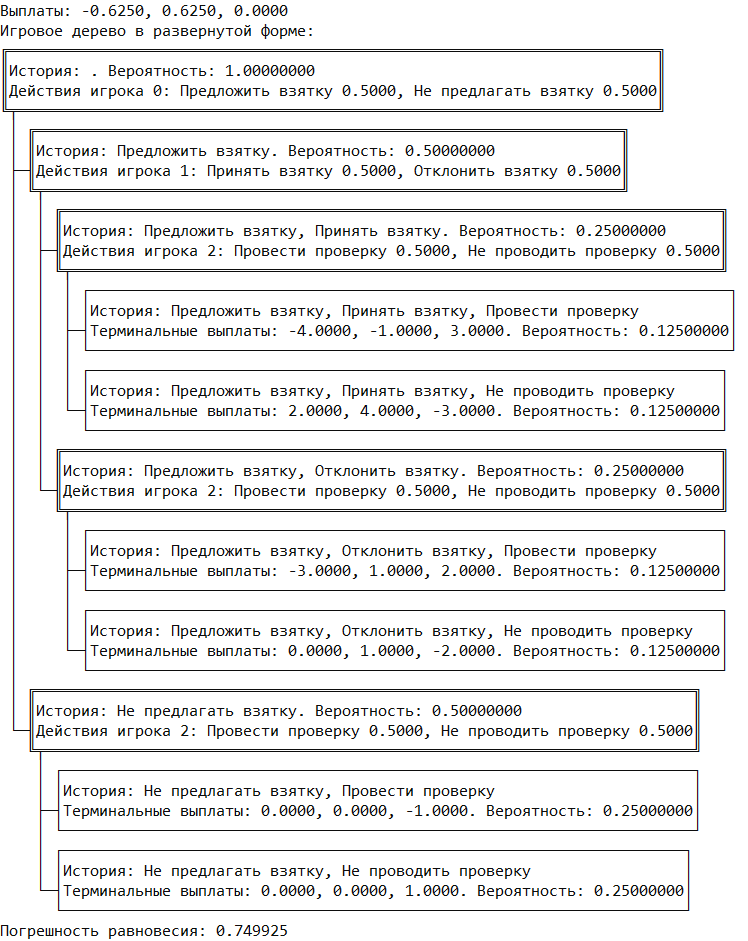
\includegraphics[width=0.9\linewidth]{inc/img/c3th11}
	\caption{Дерево игры с первой группой параметров. Случайные стратегии}
	\label{fig:c3th11}
\end{figure}

\par
На рисунке \ref{fig:c3th11} прямоугольными элементами отмечены все игровые истории, начиная с начала игры. Ребра между элементами обозначают возможные переходы между игровыми историями. Каждой нетерминальной игровой истории соответствует перечень доступных действий и стратегия их выбора. Терминальные истории сопровождаются информацией о выплатах игрокам. Для каждой истории указывается вероятность ее реализации. Расчетная эксплуатируемость данного профиля стратегий составляет примерно $0.75$. Для достижения этого значения инспектору достаточно проводить проверку с вероятностью $1.0$, изменив тем самым свой ожидаемый выигрыш с $0$ до $0.75$. Данный стратегический профиль достаточно далек от равновесия.
\par
Попробуем улучшить стратегический профиль. Проведем $T=10000$ обучающих итераций алгоритма на данном игровом дереве. Информация о обновленном стратегическом профиле представлена на рисунке \ref{fig:c3th12}.
\begin{figure}[h]
	\centering
	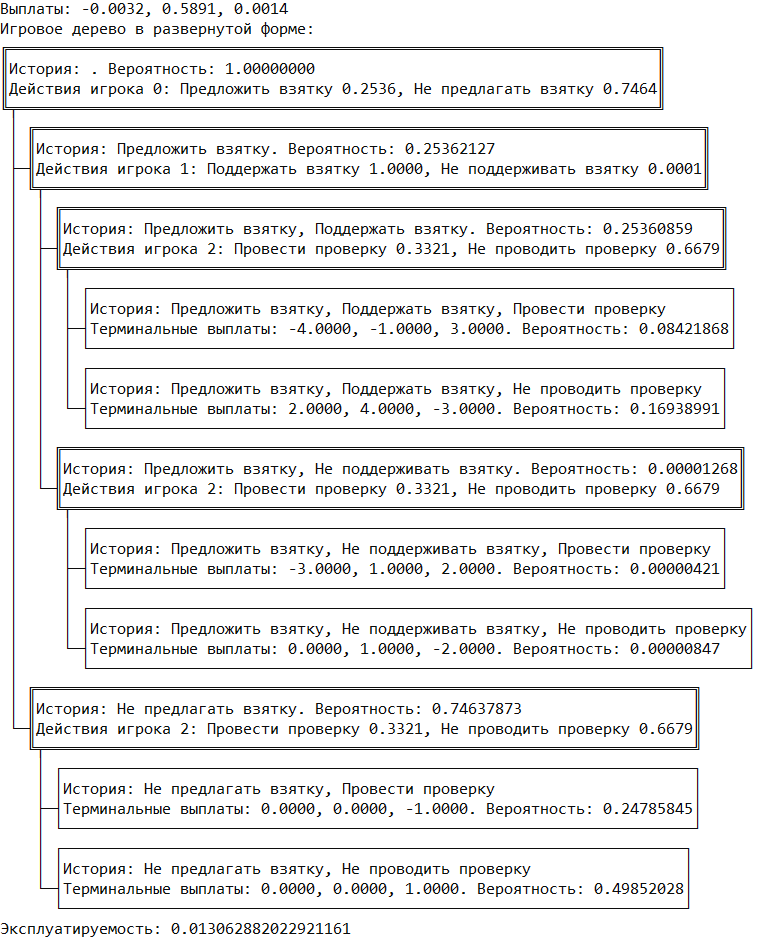
\includegraphics[width=0.9\linewidth]{inc/img/c3th12}
	\caption{Дерево игры с первой группой параметров. $T = 10000$}
	\label{fig:c3th12}
\end{figure}
\par
На рисунке \ref{fig:c3th12} отмечены выплаты, измененные стратегии игроков и измененные вероятности достижения различных игровых историй. Как можно заметить, эксплотируемость снизилась до порядка $0.01$, что сопоставимо с оценкой из теоремы \ref{CfrTStrategyExp}.
\par
Дальнейшее увеличение числа итераций приводит к снижению эксплуатируемости. График изменения расчетной эксплуатируемости для данного примера приведен на рисунке \ref{fig:c3e1}.

\begin{figure}[H]
	\centering
	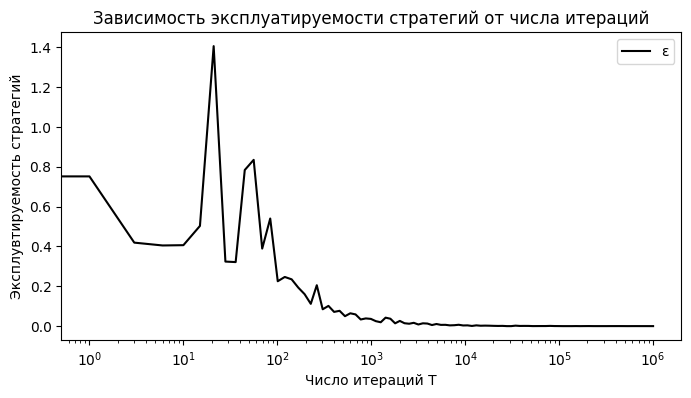
\includegraphics[width=0.8\linewidth]{inc/img/c3e1}
	\caption{Расчетная эксплуатируемость стратегий в зависимости от $T$}
	\label{fig:c3e1}
\end{figure}

\par
Рассмотрим другой набор параметров алгоритма (Таблица \ref{tbl:s1_2}).
\begin{table}[H]
	\centering
	\begin{tabular}[t]{|c|c|c|c|c|c|c|c|c|c|c|c|}
		\hline
		$v$ &	$b$ & $p_L$ &	$p_H$ & $q$ & $r$ & $\Delta x$ & $x$ & $\Delta y$ & $y$ & $\Delta z$ & $z$ \\
		\hline
		12 &	3 & 8 &	8 & 4 & 2 & 9 & 1 & 1 & 7 & 3 & 5 \\
		\hline
	\end{tabular}
	\caption{\centering Значения параметров для второго примера}
	\label{tbl:s1_2}
\end{table}
\par
Построим игровую модель и проведем $10000$ обучающих итераций. Полученный профиль стратегий представлен на рисунке \ref{fig:c3th21}.
\begin{figure}[H]
	\centering
	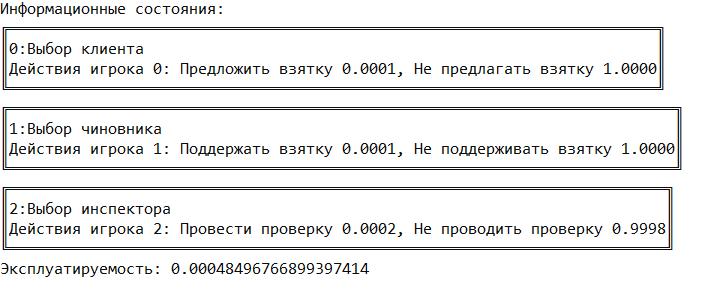
\includegraphics[width=0.8\linewidth]{inc/img/c3th21}
	\caption{Стратегии игроков для второго примера. $T=10000$}
	\label{fig:c3th21}
\end{figure}
\par
В результате мы получили профиль, который состоит из чистых стратегий. Хотя данное решение и является равновесием, оно маловероятно на практике по интуитивным соображениям. Так как алгоритм предоставляет единственное решение, имеет смысл наложить дополнительные ограничения на рассматриваемую задачу. Попробуем получить дополнительную информацию о данной игре. Для этого попробуем зафиксировать стратегию одного игрока и найти равновесие для двух оставшихся. Таким образом, найдем зависимости $\beta$ и $\gamma$ от $\alpha$, $\alpha$ и $\gamma$ от $\beta$ и зависимость $\alpha$ и $\beta$ от $\gamma$. Графики соответствующих зависимостей представлены на рисунках .

\begin{figure}[H]
	\centering
	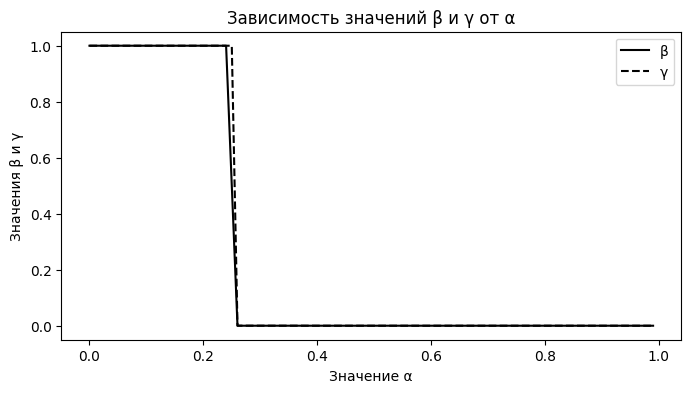
\includegraphics[width=0.8\linewidth]{inc/img/c3ex2alpha}
	\caption{График зависимости $ \beta$ и $ \gamma$ от $ \alpha$}
	\label{fig:c3ex2alpha}
\end{figure}

\begin{figure}[H]
	\centering
	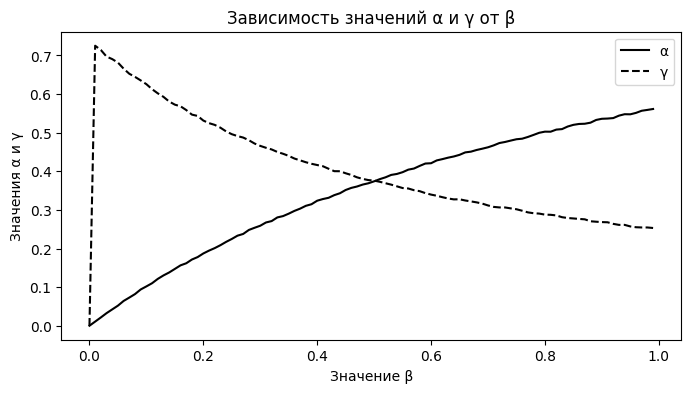
\includegraphics[width=0.8\linewidth]{inc/img/c3ex2beta}
	\caption{График зависимости $\alpha $ и $ \gamma$ от $ \beta$}
	\label{fig:c3ex2beta}
\end{figure}

\begin{figure}[H]
	\centering
	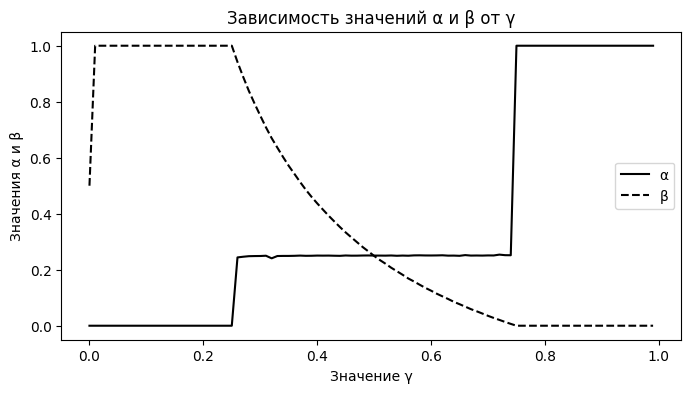
\includegraphics[width=0.8\linewidth]{inc/img/c3ex2gamma}
	\caption{График зависимости $\alpha $ и $ \beta$ от $ \gamma$}
	\label{fig:c3ex2gamma}
\end{figure}

\par
В соответствии с оценкой (\ref{eq:2.5}), вероятность проверки $\alpha$ влияет на решение чиновника о принятии взятки. В данном случае, критическое значение равно $0.25$, и на графиках \ref{fig:c3ex2alpha} и \ref{fig:c3ex2gamma} прослеживается изменение поведения участников при его преодолении инспектором.
\section{Второй пример. Модель коррупции в иерархической структуре}

В данной работе в качестве основного объекта исследования была выбрана игра «Иерархическая модель коррупции». 
	\chapter{Четвертая глава. Программная реализация цифровой подписи}
\label{cha:ch_4}
\section{Арифметические операции}
\par
В описанных ранее процессах генерации и проверки подписи часто возникает необходимость производить арифметические операции с большими целыми числами. Сложность оптимальной реализации данных процессов связана с тем, что на большинстве ЭВМ хорошо отлажены арифметические операции на ограниченном наборе типов, которые, как правило, не позволяют напрямую работать с целыми числами, занимающими более 64 бит памяти.
\par
Для реализации арифметики длинных целых чисел (более 64 бит) обычно используют специальные процедуры, работающие с конструкциями замещающими целые числа. Так, большое целое число можно представить в виде массива значений целочисленного типа, каждый элемент которого отождествляется с разрядом этого числа, как если бы оно было записанно в системе счисления с некоторым основанием. Оптимальная реализация процессов умножения или деления таких структур сама по себе является сложной задачей.
\par
Распространенность данной проблемы способствовала созданию готовых библиотек для реализации длинной арифметики в разных языках программирования. В языке C\# длинная арифметика представлена классом <<BigInteger>>. Данный класс позволяет работать с большими целыми числами, используя стандартные операторы (<<+>>, <<->>, <<*>>, <</>> и <<\%>>).
\par
Стоит отметить одну особенность данного типа, связанную с процессом формирования и проверки ЭЦП. Дело в том, что класс <<BigInteger>> содержит методы преобразования чисел в массив байт и обратно. Данные методы можно использовать для реализации процессов эквивалентных тем, что описаны в формулах (\ref{eq:bv1}), (\ref{eq:bv2}). Основным отличием является то, что в стандарте описан порядок бит от старшего к младшему, в то время как класс <<BigInteger>> предполагает порядок от младшего к старшему. В данной работе будем использовать порядок бит от младшего к старшему, для избежания лишних инверсий массивов при преобразованиях. Однако, при интеграции с внешними системами, необходимо учесть возможные инверсии. 
\section{Действия в группе точек эллиптической кривой}
\par
По аналогии с реализацией функции хэширования, выделим все свойства и методы касающиеся реализации процессов цифровой подписи в отдельный класс "--- <<GR3410\_2012\_Main>>. В качестве свойств класса определим параметры схемы цифровой подписи (пункт 4.3) и, дополнительно, добавим переменную, отражающую длину хэша "--- <<L>> (Листинг 5.1).
\lstinputlisting[caption={Параметры схемы цифровой подписи}]{inc/src/5/l51.cs}
\par
Далее определим методы, необходимые для расчета сравнений по модулю. Определим метод, вычисляющий вычет по модулю, метод, вычисляющий обратный элемент по модулю и метод, вычисляющий деление по модулю. Во втором методе, для расчета обратного элемента, используем расширенный алгоритм Евклида. Код методов представлен в Листинге 5.2.
\lstinputlisting[caption={Методы для расчета сравнений по модулю}]{inc/src/5/l52.cs}
\par
Каждую точку эллиптической кривой $Q(x,y)$ будем хранить в 2-х целочисленных переменных, отождествляемых с $x$-координатой и $y$-координатой точки. Метод, осуществляющий сложение в группе точек эллиптической кривой, определим как процедуру, принимающую координаты слагаемых точек и записывающую результат сложения в координаты третьей точки. В качестве нулевой точки $O$ возьмем точку с координатами $(-1,\;-1)$. Код метода, осуществляющего сложение в группе точек эллиптической кривой, представлен в Листинге 5.3.
\lstinputlisting[caption={Метод, осуществляющий сложение в группе точек}]{inc/src/5/l53.cs}
\par
Для получения кратных точек (\ref{eq:kP}) необходимо реализовать скалярное умножение точки эллиптической кривой на положительное целое число. Умножение должно эффективно работать с большими числами. В связи с этим, необходимо реализовать механизм быстрого умножения на скаляр по следующей формуле
\begin{equation}
kP = k_0 P + k_1 P^2 + \dots + k_n P^{2^n},\;k = \sum_{i=0}^{i=n}k_i2^i,\;k_i\in\{0,\;1\}\; i=0,\dots,n,
\end{equation} 
где $P\in E$(\ref{eq:E})$,\; k \in \mathbb{N}$.
\par
Код метода, осуществляющего умножение на скаляр в группе точек эллиптической кривой, представлен в Листинге 5.4.
\lstinputlisting[caption={Метод, осуществляющий умножение на скаляр}]{inc/src/5/l54.cs}
\section{Процесс формирования подписи}
В процессе формирования подписи необходимо генерировать случайные (псевдослучайные) числа (Шаг 3 алгоритма I). Для генерации псевдослучайных значений в рассматриваемом языке служит класс <<Random>>, экземпляры которого нужно инициализировать некоторым значением (например, текущим системным временем). Определить подобный объект в классе цифровой подписи можно следующим образом (Листинг 5.5).
\lstinputlisting[caption={Объявление генератора случайных чисел}]{inc/src/5/l55.cs}
\par
Для генерации больших случайных чисел будем использовать специальный метод, принимающий в качестве аргумента целое положительное число $p$ и возвращающий случайное число в диапазоне от $0$ до $p$ (Листинг 5.6).
\newpage
\lstinputlisting[caption={Метод для генерации случайных чисел}]{inc/src/5/l56.cs}
\par
Завершающий этап процесса генерации подписи предполагает преобразование чисел в двоичные векторы и их последующую конкатенацию (Шаг 6 алгоритма I). Данный процесс выделим в отдельный метод, учитывая специфику реализации (Листинг 5.7).
\lstinputlisting[caption={Преобразование чисел в двоичные векторы и их конкатенация}]{inc/src/5/l57.cs}
\par
Процесс формирования цифровой подписи будем осуществлять в помощью метода, принимающего в качестве аргументов хэш подписываемого сообщения и ключ подписи и возвращающего цифровую подпись. Входные и выходные значения запишем в формате массива байт. Для преобразования массива байт в числа определим специальный метод (Листинг 5.8).
\lstinputlisting[caption={Преобразование массива байт в соответствующее ему целое число}]{inc/src/5/l58.cs}
\par
Метод, осуществляющий процесс формирования подписи, представлен в Листинге 5.9. Порядок вычислений в описанном в Листинге 5.9 методе аналогичен алгоритму I.
\lstinputlisting[caption={Метод, осуществляющий процесс формирования подписи}]{inc/src/5/l59.cs}
\par
\section{Процесс проверки подписи}
В начале процесса проверки цифровой подписи необходимо получить по имеющийся подписи $\zeta$ числа $r$ и $s$ (Шаг 1 алгоритма II). Для этого, определим специальный метод, для получения чисел $r$ и $s$ по известной подписи $\zeta$ (Листинг 5.10).
\lstinputlisting[caption={Получение значений r и s из цифровой подписи}]{inc/src/5/l510.cs}
\par
Аналогично процессу формирования подписи, процесс проверки цифровой подписи оформим в виде отдельного метода, принимающего хэш подписанного сообщения, цифровую подпись и координаты ключа проверки подписи $x_q$, $y_q$. Выходным значением метода, отвечающего за проверку подписи, положим логическое значение, являющееся свидетельством достоверности подписи. Код метода проверки подписи представлен в Листинге 5.11. Порядок вычислений в описанном в Листинге 5.11 методе аналогичен алгоритму II.
\lstinputlisting[caption={Метод, осуществляющий проверку подписи}]{inc/src/5/l511.cs}
\section{Хранение параметров и значений}
В описанных ранее методах класса все глобальные методы (доступные при работе с классом вне его кода) определены относительно входных и выходных переменных, заданных массивами байт. Данный подход позволяет легко хранить данные параметры в памяти компьютера. Однако стоит заметить, что однотипность всех этих переменных может способствовать возникновению ошибок, связанных с неверным определением назначения той или иной переменной. Со структурной точки зрения более верным подходом являлось бы определение более точных типов для различных параметров алгоритма. Такой подход, в конечном итоге, упростит работу с переменными.
\par
Язык программирования C\# определяет механизмы сериализации классов в файлы формата XML, позволяющие хранить в файле не только переменные класса но и его структуру. Такой подход позволяет точно идентифицировать XML-файл как сериализованную версию экземпляра класса, что позволяет избежать подмены типов.
\par
Таким образом, определим ряд классов, отождествленных с различными параметрами процессов формирования и проверки подписи. Выделим следующие группы параметров:
\begin{itemize}
	\item параметры схемы цифровой подписи;
	\item ключ подписи;
	\item ключ проверки подписи;
	\item цифровая подпись.
\end{itemize}
\par
Каждой из выделенных групп поставим в соответствие сериализуемый класс. Список классов представлен в Листинге 5.12.
\newpage
\lstinputlisting[caption={Список классов, представляющих параметры алгоритмов}]{inc/src/5/l512.cs}
\par
Полученные классы для параметров можно использовать в классе <<GR3410\_2012\_Main>> при инициализации и при расчете процессов формирования и проверки подписи. Таким образом, определим 2 варианта конструктора класса: с использованием класса параметров схемы и без (Листинг 5.13).
\lstinputlisting[caption={2 варианта конструктора класса <<GR3410\_2012\_Main>> }]{inc/src/5/l513.cs}
\par
Вариант расчета процедур формирования и проверки подписи с использованием выделенных классов параметров представлен в Листинге 5.14.
\lstinputlisting[caption={Расчет процедур формирования и проверки подписи с использованием выделенных классов параметров}]{inc/src/5/l514.cs}
\par
Таким образом, определены все необходимые компоненты для реализации процессов проверки и генерации цифровой подписи согласно ГОСТ Р 34.10-2012. Полный код класса <<GR3410\_2012\_Main>> представлен в приложении В. В качестве практического применения разработанного класса в рамках данной работы был написан ряд вспомогательных программ, осуществляющих редактирование параметров, генерацию подписи и проверку подписи. Пример работы с данными программами представлен в приложении Г.

	
	\backmatter %% Здесь заканчивается нумерованная часть документа и начинаются ссылки и
	%% заключение
	
	\Conclusion % заключение к отчёту
\par
Реализация современных криптографических алгоритмов, безусловно, требует высокой квалификации разработчика. Это связанно с тем, что подобные алгоритмы должны работать как можно более эффективно для обеспечения быстродействия обслуживаемых ими систем. Бывает весьма трудоемко оптимальное распределение переменных по регистрам процессора и уровням кэша. Также, особого рассмотрения требует использование встроенных типов. Подобные проблемы часто бывают узкоспециализированны в зависимости от архитектуры ЭВМ и выливаются в широкий спектр прикладных вопросов.
\par
В данной работе были рассмотрены наиболее общие и надежные высокоуровневые языковые конструкции, призванные сформировать у читателя представление о процессах практического вычисления функции хэширования согласно ГОСТ Р 34.11-2012 и реализации процессов генерации и проверки ЭЦП согласно ГОСТ Р 34.10-2012.
\par
В дополнение к изложенному, в рамках данной работы был разработан ряд приложений для операционной системы Windows с графическим интерфейсом, которые позволяют непосредственно использовать описанные механизмы.
\par
Приложения реализуют:
\begin{itemize}
	\item вычисление хэш-функции от файла;
	\item редактирование параметров и ключей схемы цифровой подписи:
	\item генерацию цифровой подписи;
	\item проверку цифровой подписи.
\end{itemize}

	
	\nocite{*}
\bibliographystyle{gost780u}
\bibliography{0-main}

	
	\appendix   % Тут идут приложения
	
	\chapter{Покер Куна}
%\lstinputlisting{inc/src/appendix/Program.cs}
\chapter{Домино}
%\lstinputlisting{inc/src/appendix/Program2.cs}
	
\end{document}
